\documentclass[12pt]{article}
% \usepackage[breaklinks=true]{hyperref}
% \usepackage[html,png]{tex4ht}
\usepackage{color}
\usepackage{amsmath,amssymb,amsthm}
\usepackage{natbib}
\usepackage{array}
\usepackage{booktabs, multicol, multirow}
\usepackage[nohead]{geometry}
\usepackage[singlespacing]{setspace}
\usepackage[bottom]{footmisc}
\usepackage{floatrow}
\usepackage{float}
\usepackage{caption}
\usepackage{indentfirst}
\usepackage{lscape}
\usepackage{floatrow}
\usepackage{epsfig}
\usepackage[usenames,dvipsnames,svgnames,table]{xcolor}
\usepackage[colorlinks=true,
            urlcolor=RawSienna,
            linkcolor=RawSienna,
            citecolor=NavyBlue]{hyperref}
\floatsetup[table]{capposition=top}
\floatsetup[figure]{capposition=top}


\newcommand{\cD}{{\mathcal D}}
\newcommand{\cF}{{\mathcal F}}
\newcommand{\todo}[1]{{\color{red}{TO DO: \sc #1}}}

\title{Student Evaluations of Teaching (Mostly) Do Not Measure Teaching Effectiveness}
\author{Anne Boring, Kellie Ottoboni, Philip B.~Stark}
\date{Draft \today}
\begin{document}
\maketitle

\newpage
\begin{quotation}
    \emph{The truth will set you free, but first it will piss you off.}
    
     \hfill Gloria Steinem

\begin{abstract}
We examine student evaluations of teaching (SET) at SciencesPo
University, Paris, where all
first-year students take the same courses 
(economics, history, political science, sociology, and political institutions). 
Students are assigned to sections of those courses as if at random, creating a natural experiment.
Final exams are set for the entire course
by the professor rather than the section instructor, and are graded anonymously.
Hence, final exam scores are a proxy for the effectiveness of the section instructors.
SET are mandatory.
We study relationships among SET and the genders of students and
instructors, topic, final exam scores, and students' grade expectations
for 23,001 SETs of 379 instructors by 4,423 students over five years.
Nonparametric permutation tests that aggregate within the 1,194 course sections show: 
\begin{itemize}
   \item the association between SET and final 
            exam scores is negative but insignificant
            ($P \approx 0.70$)
   \item the association between SET and grade 
            expectations is positive and highly significant
            ($P \approx 0.00$)
   \item the association between instructor gender 
            and final exam scores is insignificant
            (students of male instructors do worse, $P \approx 0.51$ overall, $0.76$ 
            for male students, $0.65$ for female students)
   \item the association between instructor gender and SET is highly significant---because male
             students rate male instructors higher 
            (men get higher ratings, $P \approx 0.00$ overall, $0.00$ for male students,
            $0.49$ for female students)
\end{itemize}
These relationships vary by discipline.
%Student responses fail simple tests of data quality.
%For instance, 29\% of students report spending impossible amounts of time
%on their courses.

\end{abstract}

\newpage

\end{quotation}

\section{Background}
Student evaluations of teaching (SET) are used widely in higher education 
as a measure of teaching quality,
and figure in the hiring, promotion, and firing of instructors, especially non-tenured faculty.
SET are generally treated as a measure of teaching effectiveness, rather than, e.g., a measure of student satisfaction.
Because ascertaining teaching effectiveness is so difficult---for students,
faculty, and administrators alike---attempts to measure teaching effectiveness by
surveying student opinion may suffer from conscious or unconscious biases. 
Recent work by \citet{MacNell2014} has demonstrated that this is the case: 
their randomized, controlled experiment shows that, on average, students rate a given instructor
lower on every aspect of teaching (including ``objective'' measures such as
timeliness) when they think the instructor is female than when 
they think the instructor is male.

Randomized, controlled experiments also show that SET do not measure
teaching effectiveness; the key studies are \citet{Carrell2010a,Braga2014},
which find that students confuse grades (or grade expectations) with long-term
value.

Here, we use a remarkable census of SET by first-year students at SciencesPo (Paris)
collected between 2008 and 2013, 
comprising 22,665 SETs by
4,423 students (57\% women) of 1,177
sections and  taught by 372 instructors (33\% women)\footnote{The data include SET scores for the six first year mandatory courses, i.e. history, political institution, microeconomics, macroeconomics, political science and sociology}.
These data are discussed in detail by \citet{Boring2015}.
The key aspects of the data are these:
\begin{itemize}
   \item All first year students take the same six courses, in history, macroeconomics, microeconomics, 
            political institutions, political science, and sociology.
            Each course has one main professor,
            who delivers the lectures (to groups of approximately 900 students) and creates 
            the final exams.
            Courses have many sections of 10--24 students. 
            Those sections are taught by different instructors.
            The instructors have considerable pedagogical freedom.
    
   \item Students enroll in ``triads'' of sections of these courses. 
            The enrollment process
            does not allow students the freedom to select individual instructors.
            The assignment of students to sections is ``as if'' at random.
            
   \item Section instructors provide interim grades during the term. 
            Students know what their interim grades are, so interim grades are a 
            good measure of grade expectations.
            
   \item Final exams are set by the main professor: all students in a given course take the
            same final. Final exams are graded anonymously in all disciplines except Political
            Institutions (which we omit from analyses involving final exam scores).
            This makes performance on the final exam a reasonable measure of the value the
            section instructor adds: students of more effective instructors should do better on
            the final exam, on average.
    
   \item SET are mandatory: the response rates are nearly perfect.
   
\end{itemize}

SETs include closed-ended and open-ended questions, 
but the question that attracts the most attention is the overall 
score, which is considered to be a summary 
of the scores on the other questions. 


Our SET data include students' individual evaluations of instructors in the sections for microeconomics, history, political institutions, and macroeconomics for the five academic years 2008--2013, and for sociology and political science courses for the three academic years 2010--2013 
(these two were introduced in 2010). Students have been completing their SETs online since 2008. The SET scores are
anonymous to the teachers, who only have access to them once all grades have been officially recorded on student transcripts, several weeks after final exams. Instructors and academic coordinators then have access to SETs. When scores are low, the academic coordinator discusses the SETs with the instructor.   
 


\begin{table}[htbp]
  \centering
  \footnotesize 
  \caption{Descriptive statistics of instruction sections}
    \begin{tabular}{lccc}
    \toprule 
                        & N. courses & N. instructors  & \% Female instructors  \\
   \midrule
  \textbf{Overall} &  \textbf{1,194} & \textbf{379}  &\textbf{33.8\%} \\
    History    &               230 &      72          &   30.6\% \\
    Political institutions  &  229 &      65          &   20.0\% \\    
    Microeconomics   &         230 &      96          &   38.5\% \\
    Macroeconomics   &         230 &      93          &   34.4\% \\
    Political science &       137 &      49          &   32.7\% \\
    Sociology   &              138 &      56          &   46.4\%    \\
    \bottomrule
    \end{tabular}%
 \label{tab:description}%
 
\textit{Note: the data for one political institutions section were excluded as this section had an experimental online format. The political science and sociology courses were originally not included in the triad system, and students were randomly assigned by the administration to different sections.} 

\end{table}%
\normalsize

While 33.8\% of the 1,194 instruction sections are taught by women (table \ref{tab:description}), there is some variation by discipline. The political institutions sections are the ones more often taught by men (only 20\% are taught by women). The sociology sections are almost equally divided between male and female instructors (46.4\% are taught by women).  




We investigate 
hypotheses relating to whether the overall satisfaction score  primarily measures teaching
effectiveness or something else, for instance, the gender of the instructor or students'
grade expectations.
The data also allow us to determine whether there are systematic differences
in how students rate courses in different disciplines.

We use nonparametric permutation tests rather than, for instance, logistic regression.
Using nonparametric tests allows us to avoid counterfactual assumptions about
generative models for the data, which regression-based methods (including
ordinary linear regression, mixed effects models, logistic regression, etc.) and parametric
methods such as $t$-tests and ANOVA, would require.
The null hypotheses for our tests are simply that some 
characteristic---e.g., instructor gender---amounts to an arbitrary label, and might as well
have been assigned at random. 

Our analysis is conducted at the level of courses, which matches how SET are
used in practice by institutions: typically, student responses in a given course
are averaged, and those averages are compared across instances of the course,
across courses in a department, and across departments within a university.
Some of the statistical issues in this reduction of SET to averages are 
discussed by \citet{Stark2014}

To further the analysis on the validity of SET scores as a measure of teaching effectiveness, we
also use nonparametric permutation tests on the data from \citet{MacNell2014}. We find similar results: 
SET scores primarily do not measure teaching effectiveness. Gender biases are a strong determinant of SET scores.


\section{Tests}
In this section, we provide the results of different nonparametric tests, whose purpose is to analyze the validity and reliability of SETs. 





\subsection{The correlation between SET scores and student performance}

Teaching effectiveness is multidimensional (e.g. \citet{Marsh1997}), and can therefore be difficult to measure. However, effective teaching should generate student learning, suggesting that effective instructors should lead their students to learn and understand more course material. Effective instructors should therefore cause their students to obtain higher grades, on average. 

We first test whether SET scores are correlated with higher grades on the final exam, on average by section (Table \ref{tab:finalexam}). The results suggest that SET scores do not always measure actual teaching effectiveness. 

\begin{table}[htbp]
  \centering
  \footnotesize 
  \caption{Correlation between average SET scores and final exam grades, by course number}
    \begin{tabular}{lcc}
    \toprule 
                        & $\rho$  & $p$-value  \\
   \midrule
    Overall &            -0.02 &       0.70  \\
    History &             0.03 &       0.31  \\
    Macroeconomics &      0.12 &       0.04  \\
    Microeconomics &      0.13 &       0.03  \\
    Political science & -0.01 &       0.53  \\
    Sociology &           0.05 &       0.27  \\
    \bottomrule
    \end{tabular}%
 \label{tab:finalexam}%
 
  \textit{Note: one-sided $p$-values are reported.}
\end{table}%
\normalsize




\subsection{The correlation between SET scores and gender}


Although uncorrelated with students’ performance on the final exam, SETs appear to be much better predictors of gender. Overall, average SET scores and instructor gender are correlated, with male instructors obtaining significantly higher SET scores ($p$-value of 0.00). There are, however, strong variations by course type (Table \ref{tab:instructorgender}). Male instructors of history, macroeconomics and political institutions courses receive significantly higher overall satisfaction scores ($p$-values of 0.07, 0.08 and 0.10 respectively). The relationship is also positive between SET scores and instructor gender for microeconomics, political science and sociology courses, although not significantly ($p$-values of 0.58, 0.43 and 0.26 respectively).   

\begin{table}[htbp]
  \centering
  \footnotesize 
  \caption{Analyzing the correlation between average SET score and instructor gender, by course}
    \begin{tabular}{lcc}
    \toprule 
                          & $\rho$  & $p$-value     \\
   \midrule
    Overall &                 0.10       & 0.00     \\
    History &                 0.12       & 0.07     \\
    Political institutions &  0.11       & 0.10     \\
    Macroeconomics &          0.11       & 0.08     \\
    Microeconomics &          0.04       & 0.58     \\
    Political sciences &      0.07       & 0.43     \\
    Sociology &               0.10       & 0.26     \\
    \bottomrule
    \end{tabular}%
 \label{tab:instructorgender}%
  
  \textit{Note: two-sided $p$-values are reported.}
\end{table}%
\normalsize


Do men receive higher SET scores overall because they are better instructors? If men were indeed better instructors, then their students should perform better on the final exam. This is not the case, however (Table \ref{tab:genderfinal}). Indeed, the correlation between student performance and instructor gender is negative, although statistically insignificant ($p$-value of 0.51 overall). 



\begin{table}[htbp]
  \centering
  \footnotesize 
  \caption{Correlation between final exam average and instructor gender, by course}
    \begin{tabular}{lcc}
    \toprule 
                     & $\rho$  & $p$-value    \\
   \midrule
    Overall &            -0.02       & 0.51      \\
    History &            -0.06       & 0.39      \\
    Macroeconomics &      0.00       & 0.97      \\
    Microeconomics &     -0.03       & 0.63      \\
    Political sciences &  0.02       & 0.79      \\
    Sociology &          -0.00       & 0.97      \\
    \bottomrule
    \end{tabular}%
 \label{tab:genderfinal}%
 
  \textit{Note: two-sided $p$-values are reported.}
\end{table}%
\normalsize



SET scores and instructor gender are correlated, because male students tend to give higher Set scores to male instructors (Table \ref{tab:genderconcordance}). Gender concordance is a statistically strong predictor of SET scores for men ($p$-value of 0.00 overall). Male students give higher SET scores to male instructors in all fields. The correlations are statistically significant in history ($p$-value of 0.00), political institutions ($p$-value of 0.07), macroeconomics ($p$-value of 0.04), microeconomics ($p$-value of 0.10) and political science ($p$-value of 0.06). The correlation is positive although statistically insignificant in sociology ($p$-value of 0.15), i.e. the field in which the proportion of female instructors is the highest. 

Although gender concordance is correlated with overall satisfaction scores for male students, SET scores of female students are not statistically correlated with instructor gender ($p$-value of 0.49 overall). The correlation is negative in some fields (history, political institutions, macroeconomics and sociology) and positive in others (microeconomics and political science), but always statistically insignificant ($p$-values between 0.19 and 0.97).



\begin{table}[htbp]
  \centering
  \footnotesize 
  \caption{Correlation between SET scores and gender concordance}
    \begin{tabular}{lcc}
    \toprule 
                          & $\rho$  & $p$-value   \\
   \midrule
     \multicolumn{3}{l}{\textit{Male students}} \\     
      \quad  Overall &                 0.15       & 0.00       \\
      \quad  History &                 0.18       & 0.00       \\
      \quad  Political institutions &  0.12       & 0.07        \\
      \quad  Macroeconomics &          0.14       & 0.04        \\
      \quad  Microeconomics &          0.11       & 0.10        \\
      \quad  Political sciences &      0.16       & 0.06       \\
      \quad  Sociology &               0.12       & 0.15       \\
   \midrule
     \multicolumn{3}{l}{\textit{Female students}} \\     
      \quad  Overall &                  0.02       & 0.49      \\
      \quad  History &                 -0.04       & 0.54       \\
      \quad  Political institutions &  -0.09       & 0.19       \\
      \quad  Macroeconomics &          -0.08       & 0.21       \\
      \quad  Microeconomics &           0.03       & 0.67       \\
      \quad  Political sciences &       0.00       & 0.97       \\
      \quad  Sociology &               -0.05       & 0.53       \\
    \bottomrule
    \end{tabular}%
 \label{tab:genderconcordance}%
  
  \textit{Note: two-sided $p$-values are reported.}
\end{table}%
\normalsize




Do male instructors receive higher SET scores from male students because their teaching styles match male students’ learning styles?\footnote{Discussion about whether learning styles exist?} If that were the case, then male students who had male instructors should perform better on the final exam. However, this is not the case (Table \ref{tab:finalconcordance}). If anything, male students who had male instructors appear to perform worse overall on the final exam (the correlation is statistically insignificant, with a $p$-value of 0.76). In history, the negative correlation is weakly statistically significant ($p$-value of 0.10). Although in history male students give significantly higher SET scores to male instructors, they perform worse on the final exam when they had a male instructor, suggesting that students are not measuring teaching effectiveness when they complete their SETs. 




\begin{table}[htbp]
  \centering
  \footnotesize 
  \caption{Student performance and gender concordance}
    \begin{tabular}{lcc}
    \toprule 
                          & $\rho$  & $p$-value   \\
   \midrule
     \multicolumn{3}{l}{\textit{Male students}} \\     
      \quad  Overall &                 -0.01       & 0.76      \\
      \quad  History &                 -0.11       & 0.10      \\
      \quad  Macroeconomics &           0.02       & 0.76      \\
      \quad  Microeconomics &          -0.04       & 0.60      \\
      \quad  Political sciences &       0.10       & 0.25      \\
      \quad  Sociology &                0.02       & 0.85      \\
   \midrule
     \multicolumn{3}{l}{\textit{Female students}} \\     
      \quad  Overall &                  0.01       & 0.65        \\
      \quad  History &                  0.01       & 0.86        \\
      \quad  Macroeconomics &          -0.00       & 0.97        \\
      \quad  Microeconomics &           0.00       & 0.94      \\
      \quad  Political sciences &       0.03       & 0.76        \\
      \quad  Sociology &               -0.01       & 0.94        \\
    \bottomrule
    \end{tabular}%
 \label{tab:finalconcordance}%
  
  \textit{Note: two-sided $p$-values are reported.}
\end{table}%
\normalsize





\subsection{The correlation between SET scores and grade expectations}

SET scores are strongly correlated with grade expectations.   



\begin{table}[htbp]
  \centering
  \footnotesize 
  \caption{Analyzing the correlation btw avg evaluation score and cont assessment, by course number}
    \begin{tabular}{lcc}
    \toprule 
                          & $\rho$  & $p$-value  \\
   \midrule
    Overall &                 0.10       & 0.00   \\
    History &                 0.32       & 0.00   \\
    Political institutions &  0.06       & 0.19     \\
    Macroeconomics &          0.22       & 0.00    \\
    Microeconomics &          0.19       & 0.00     \\
    Political sciences &      0.16       & 0.03     \\
    Sociology &               0.27       & 0.00     \\
    \bottomrule
    \end{tabular}%
 \label{tab:instructor gender}%
  
  \textit{Note: one-sided $p$-values are reported.}
\end{table}%
\normalsize



Discuss correlation between continuous assessment and final exam grades? 



For microeconomics, gender concordance for male students and instructors is only weakly correlated with SETs ($p$-value of 0.10). Several reasons can explain this result. First, the microeconomics course   


While the focus of this paper has been to question the validity of SETs as measures of teaching effectiveness, by showing that gender is a stronger predictor of SET scores than student performance, the academic research on SETs suggests that reliability may also be an issue.

\begin{figure}
\begin{centering}
  \caption{Proba}
  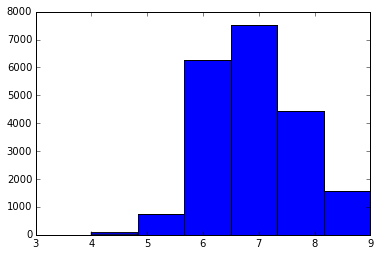
\includegraphics[height=3in]{reliability}
\end{centering}
\end{figure}


Using the data from Sciences Po, we check for the reliability of students answers. 



\section{Student bias or preference for male instructors?}

Bias or preference? It seems to be a bias, since male students do not perform better on the final exam with male instructors. However, they nonetheless may have a preference for male instructors. 

Controlling for teaching style can help differentiate between bias and preference. We know of two experiments which were able to control for teaching styles (\citet{Arbuckle2003} and \citet{MacNell2014}).  

\citet{Arbuckle2003}: what they do...  


\citet{MacNell2014}: what they do...  


For the purpose of this paper, we also used permutation tests to analyze the data provided by \citet{MacNell2014}. We find similar results as in their analysis...


\section{Code}
Github repo. \url{https://github.com/kellieotto/SET-and-Gender-Bias}

\section{Discussion}

The tests that we have performed sugges that it is impossible to know what SETs are measuring at what time. 




\subsection{What is teaching effectiveness?}

Implicit in the use of SET as a 
Push back on the notion of ``teaching effectiveness.''
There ought to be \emph{some} interaction between characteristics of the
instructor and those of the student.
If ``effectiveness'' is intrinsic to the instructor, ratings in one class shouldn't depend on
which other classes a student takes.
Looking at ratings ``per student'' doesn't make sense if you are trying to
measure some underlying platonic ``effectiveness'' intrinsic to the instructor.
In particular,  a showing that individual students who give a particular instructor higher ratings
get higher grades, does not point to ....\todo{fix me}

Teaching effectiveness is a vague notion that even researchers of higher education have a hard time defining. 

The notion of teaching effectiveness implies that instructors have some control over the impact their teaching skills have on student-related outcomes. Measures of teaching effectiveness should therefore only reflect variables that are under the control of instructors. Instead of measuring teaching effectiveness, SETs are a measure student satisfaction regarding a course \citep{Stark2014}. Students may be satisfied or dissatisfied with courses for reasons outside of the control of instructors.   

Gender is not the only variable unrelated to teaching effectiveness that other studies have shown to be predictors of SET scores. Given the many variables that are likely to bias SET scores and whose weight in SETs are likely to change from one learning environment to another, it would be impossible to control for these variables to make SETs a reliable and valid measure of teaching effectiveness. 

Among the instructor characteristics alongside gender, race has also been shown to be correlated with SET scores.  In studies conducted in the U.S. context, instructors of color appear to suffer from student biases similar to those that female instructors suffer from. Minority instructors tend to receive significantly lower SET scores compared to white (male) instructors (e.g. \citet{Merritt2008}).\footnote{French law does not allow for the use of race-related variables in data sets. We were thus unable to test for potential racial biases in SET scores in the context of SciencesPo.} 

Other instructor-related characteristics likely to be unrelated to teaching effectiveness have been shown to be predictors of SET scores, such as age, charisma \citep{Shevlin2000}, physical attractiveness (e.g. \citet{Riniolo2006} and \citet{Hamermesh2005}).  

Variables related to student characteristics.

Variables related to the course being taught. mathematical difficulty

Other factors still unrelated to factors that an instructor can control appear to be related to SET scores.  Variables related to the teaching environment, class time, class size

Hill2010: Students noted differences in the physical characteristics of classrooms, including the seating characteristics, lighting, desk space, and noise levels. Overall, these differences affected the students' perceptions of the instructors' organization, their own enjoyment of the class, their perceived level of learning, and their general sense of satisfaction


Hundreds of studies discuss and question the validity of SETs as a measure of teaching effectiveness (e.g. for reviews \citep{Pounder2007}). Some studies find results that are similar to ours, with male students expressing biases in favor of male instructors (e.g. \citet{Basow1987}; \citet{Kaschak1978}). Other studies find that the correlation between gender and SETs is uncorrelated or weak (e.g. \citet{Bennett1982}; \citet{Centra2000}; \citet{Elmore1974}). 
While some studies tend to suggest that SETs are not a valid measure of teaching effectiveness {e.g. \citet{Galbraith2012} and \citep{Carrell2010a}), others argue that SETs are valid and reliable measures of teaching effectiveness (e.g. \citet{Benton2012} and \citet{Centra1977}). While there is no consensus among academics on the issue of validity, the fact that different studies show such a wide variety of results suggests that validity varies with contexts. This fact, in itself, shows that SETs are not universally valid and should be used by universities with caution. 



\section{Conclusions}

The correlation between SET and performance isn't zero:
it is positive, albeit not statistically significant. The larger point is that SETs are better measures of student grade expectations and of instructor gender than they are of teaching effectiveness. The results we find suggest that female instructors may receive lower than average SET scores, despite being as effective instructors as men, only because of student biases in favor of male instructors. The use of SETs therefore unfairly penalizes women, and can have large consequences on their academic careers. 

In the US, SETs have two purposes: 1) to help instructors improve their teaching skills, and 2) to help the administration decide on the hiring or promotion of instructors. We guard against the use of SETs for this second purpose, given the biases that may strongly influence students in the overall satisfaction scores. In fact, in France, the French Ministry of Higher Education and Research upheld in 2009 a 1997 decision of the French State Council which stated that public universities can only use SETs to help instructors improve their pedagogy, but members of the administration are not allowed to use SETs as a tool for making decisions which might affect instructors' careers (cf. \citet{Boring2015a}. 

SETs tend to measure student satisfaction, and not actual teaching effectiveness. As others have already suggested in the literature, alternatives to SETs...  


\bibliographystyle{abbrvnat}
\bibliography{SETs}

\end{document}

